\documentclass[11pt,xcolor={dvipsnames},aspectratio=159,hyperref={pdftex,pdfpagemode=UseNone,hidelinks,pdfdisplaydoctitle=true},usepdftitle=false]{beamer}
\usepackage{presentation}[aspectratio=169]
\usepackage{math}
\usepackage{mathtools}
\usepackage{mleftright}
% Enter title of presentation PDF:
\hypersetup{pdftitle={Government Spending Multiplier: Theory I}}
% Enter link to PDF file with figures:

\begin{document}
% Enter presentation title:
\title{Government Purchases Multiplier: Theory I}
\subtitle{Fiscal and Monetary Policy 2026}
% Enter presentation information:

% Enter presentation authors:
\author{Piotr Żoch}%
% Enter presentation location and date (optional; comment line if not needed):
\frame{\titlepage}

% Fill out content of presentation:

\begin{frame}
    \heading{Old (?) Keynesian multiplier}
\end{frame}

\begin{frame}{Keynesian multiplier}
    \begin{itemize}
    \item Recall your undergraduate macroeconomics course.
    \item A simple model of a closed economy \begin{align*}
        Y_t &= C_t + I_t + G_t \\
        C_t &= \a_0 + \a_1 \bp{Y_t - T_t} \\
        I_t &= I_0 
    \end{align*}
    where $Y_t$ is output, $C_t$ is consumption, $I_t$ is investment, $G_t$ is government purchases of goods and services and $T_t$ is taxes.
    \item We \emph{assume} consumption in period $t$ is a function of disposable income in period $t$ and investment is exogenous.
    \item Here $a_1 \in\bp{0,1}$ is \emph{the marginal propensity to consume}.  
    \end{itemize}
\end{frame}

\begin{frame}{Keynesian multiplier}
    \begin{itemize}
    \item We can solve for equilibrium output $Y_t$: \begin{align*}
        Y_t = \frac{1}{1 - a_1} \bs{\a_0 + I_0 + G_t - a_1 T_t}
    \end{align*} 
    \item The \alg{government spending multiplier} is \begin{align*}
        \frac{\partial Y_t}{\partial G_t} = \frac{1}{1 - a_1}.
    \end{align*}
    \item The size of the multiplier depends on the marginal propensity to consume. Notice the multiplier is \alr{always} larger than one because $a_1 > 0$.
    \end{itemize}
\end{frame}


\begin{frame}{Keynesian multiplier}
    \begin{itemize}
    \item The result above relied on the assumption that $T_t$ is constant. What if it is not?
    \item Suppose $T_t = G_t$ (balanced budget). We then have \begin{align*}
        \frac{\partial Y_t}{\partial G_t} = 1.
    \end{align*}
    \item Notice that the multiplier is now equal to one regardless of the value of $a_1$.
    \item Haavelmo (1945) showed this result. 
    \end{itemize}
\end{frame}

\begin{frame}{Taking stock}
    \begin{itemize}
    \item Even if the government spends exactly as much as it collects in taxes, output will increase one to one. 
    \item If the government spends more than it collects in taxes, output will increase by more than one to one.
    \item The multiplier is larger than one because of the marginal propensity to consume greater than zero.
    \end{itemize}
\end{frame}

\begin{frame}{Taking stock}
    \begin{itemize}
    \item Too good to be true?  
    \item What are the limitations of this model?
    \item What determines the key parameter $a_1$?
    \item Similar results tend to hold in more complex models (see ``The Intertemporal Keynesian Cross'' by Auclert, Rognlie, and Straub, JPE 2024).
    \item We will first study government purchases multiplier in a benchmark model -- the Neoclassical Growth Model. 
    \end{itemize}
\end{frame}

\begin{frame}
    \heading{Neoclassical Growth Model - recap}
\end{frame}

\begin{frame}{NGM: household}

\begin{itemize} 
    
    \item Representative household chooses $\left\{ c_{t},n_{t},k_{t+1}\right\} _{t=0}^{\infty}$
    to maximize 
    \[
    \sum_{t=0}^{\infty}\beta^{t}\left[u\left(c_{t}\right)-v\left(n_{t}\right)\right]
    \]
     subject to
    \begin{align*}
    c_{t}+\underbrace{k_{t+1}-\left(1-\delta\right)k_{t}}_{i_{t}} & =w_{t}n_{t}+r_{t}^{k}k_{t}\quad\text{for all }t\geq0
    \end{align*}
    given $k_{0}$.
    
    \begin{itemize}
    \item $u\left(\cdot\right)$ strictly increasing, $C^{2}$, strictly concave,
    $u'\left(0\right)=\infty$, $u'\left(c\right)_{c\rightarrow\infty}=0$;
    \item $v\left(\cdot\right)$ strictly increasing, $C^{2}$, strictly convex,
    $v'\left(n\right)_{n\rightarrow\infty}=\infty$.
    \end{itemize}
\end{itemize}    
\end{frame}


\begin{frame}{NGM: firm}

    \begin{itemize} 
        \item Representative producer chooses $\left\{ y_{t},k_{t},n_{t}\right\} _{t=0}^{\infty}$
    to maximize 
    \[
    y_{t}-r_{t}^{k}k_{t}-w_{t}n_{t}\quad\text{for all }t\geq0
    \]
    subject to 
    \[
    y_{t}=F\left(k_{t},n_{t}\right)\quad\text{for all }t\geq0.
    \]
    \begin{itemize}
    \item $F\left(\cdot,\cdot\right)$ is CRtS, concave, increasing
    and satisfies Inada conditions.
    \end{itemize} 
\end{itemize}
    \end{frame}

\begin{frame}{NGM: competitive equilibrium}

       \begin{itemize}
        \item \textbf{Competitive Equilibrium: }sequence of prices and allocations
such that:
\begin{itemize}
\item Households maximize utility subject to their budget constraints given
prices;
\item Firms maximize profits subject to their production sets given prices;
\item All markets clear: 
        $$y_{t}=c_{t}+k_{t+1}-\left(1-\delta\right)k_{t}$$
        (+ labor and capital market -- by using the same variable for
        demand and supply).
\end{itemize}
\end{itemize}
        \end{frame}

    %
    \begin{frame}{NGM: characterization}
    \begin{itemize}
    \item Lagrangian for the household problem: 
    \[
    \sum_{t=0}^{\infty}\beta^{t}\left[u\left(c_{t}\right)-v\left(n_{t}\right)\right]+\lambda_{t}\left[w_{t}n_{t}+r_{t}^{k}k_{t}-c_{t}-k_{t+1}+\left(1-\delta\right)k_{t}\right]
    \]
    \item First order conditions 
    \begin{align*}
    \beta^{t}u'\left(c_{t}\right) & =\lambda_{t}\\
    \beta^{t}v'\left(n_{t}\right) & =\lambda_{t}w_{t}\\
    \lambda_{t} & =\lambda_{t+1}\left(1-\delta+r_{t+1}^{k}\right)
    \end{align*}
    \end{itemize}
    \end{frame}


\begin{frame}{NGM: characterization}
    \begin{itemize}
    \item Solution to the household's problem described by the following: 
    \begin{align*}
        u'\left(c_{t}\right) & =\beta u'\left(c_{t+1}\right)\left(1-\delta+r_{t+1}^{k}\right)\\
        v'\left(n_{t}\right) & =u'\left(c_{t}\right)w_{t},
        \end{align*}
    the budget constraint $$c_{t}+k_{t+1}-\left(1-\delta\right)k_{t}=w_{t}n_{t}+r_{t}^{k}k_{t},$$ the initial condition ($k_0$ given), and the transversality condition $$\lim_{t\to\infty}\beta^{t}u'\left(c_{t}\right)k_{t+1}=0.$$   
    \end{itemize}
    \end{frame}    
    


\begin{frame}{NGM: characterization}
    \begin{itemize}
    \item Solution to the firm's problem described by the following: 
    \begin{align*}
        r_{t}^{k} & =F_{1}\left(k_{t},n_{t}\right)\\
        w_{t} & =F_{2}\left(k_{t},n_{t}\right),
        \end{align*}
    and the production function $$y_{t}=F\left(k_{t},n_{t}\right).$$
    \end{itemize}
    \end{frame}    

\begin{frame}{NGM: characterization}
    \begin{itemize}
    \item \textbf{Equilibrium conditions}: 
    \begin{align}
    u'\left(c_{t}\right) & =\beta u'\left(c_{t+1}\right)\left[1-\delta+F_{1}\left(k_{t+1},n_{t+1}\right)\right]\tag{EE}\label{EE}\\
    v'\left(n_{t}\right) & =u'\left(c_{t}\right)F_{2}\left(k_{t},n_{t}\right)\tag{LS}\label{LS}\\
    k_{t+1} & =F\left(k_{t},n_{t}\right)+\left(1-\delta\right)k_{t}-c_{t}\tag{LoM}\label{LoM}
    \end{align}
    + the transversality condition which pins down the solution, and the initial condition ($k_0$ given).     
    \item Sequences of $\bc{c_t, n_t, k_t}$ that satisfy these conditions constitute allocations in a competitive equilibrium. 
\end{itemize}
    
    \end{frame}        
    
\begin{frame}{Comments}
    \begin{itemize}
    \item Tradeoffs in the model:
    \begin{itemize}
    \item consumption today $c_{t}$ vs. consumption tomorrow $c_{t+1}$;
    \item consumption vs. leisure.
    \end{itemize}
    \end{itemize}
    \end{frame}


    \begin{frame}
        \heading{Neoclassical Growth Model - government purchases}
    \end{frame}

\begin{frame}{Government purchases}
    \begin{itemize}
    \item We add government purchases, $g_{t}$ to the model.
    \item They do not affect utility, they just use up $g_{t}$ units of goods
    each period.
    \item They are financed by lump-sum taxes: $T_{t}=g_{t}$ in each period.
    \item BC of the HH is: 
    \[
    c_{t}+i_{t}=w_{t}n_{t}+r_{t}^{k}k_{t}-\al{T_t}\quad\text{for all }t\geq0.
    \]
    \item Market clearing condition is: 
    \[
    c_{t}+i_{t}+\al{g_t}=y_{t}.
    \]
    \item Note: in this model it does not matter if the budget is balanced or $g_t$ is financed by debt, as long as taxes are lump-sum (\alg{Ricardian equivalence}). 
    \end{itemize}
    \end{frame}
    %
    \begin{frame}{Multiplier}
    \begin{itemize}
    \item Questions we might want to answer:
    \begin{itemize}
    \item effects of a permanent change in (constant) $\bar{g}$ in the steady
    state;
    \item effects of an unexpected change and transitory in $g_{t}$ on impact
    (i.e. in period $t$);
    \item cumulative effects of a change in $g_{t}$; 
    \item effects of a pre-announced change in $g_{t}$...
    \end{itemize}
    \end{itemize}
    
    \end{frame}

    \begin{frame}{Multiplier - long run}
        \begin{itemize}
        \item We first discuss the long-run effect of permanent changes (steady state).
        \item Define $\eta\coloneqq k \slash n$.
        \item By CRtS we have $F\left(k,n\right)=F\left(\eta,1\right)n$ and $F_{1}\left(k,n\right)=F_{1}\left(\eta,1\right)$.
        \item The Euler equation in the steady state is: 
        \begin{align*}
            1 = \beta\left[1-\delta+F_{1}\left(\eta,1\right)\right]\tag{EE}\label{EE-1-1}
        \end{align*}
        which pins down $\eta$. 
        \end{itemize}
        \end{frame}


    \begin{frame}{Multiplier - long run}
        \begin{itemize}
        \item The other two equations (labor supply and law of motion for capital) give us a system of two equations in two unknowns, $c$ and $n$:
        \begin{align}
        v'\left(n\right) & =u'\left(c\right)\al{F_{2}\left(\eta,1\right)}\tag{LS}\label{LS-1-1}\\
        c & =\left(\al{F\left(\eta,1\right)-\eta\delta}\right)n-\al{g}\tag{LoM}\label{LoM-1-1}
        \end{align}
        \item Given our assumptions we can rewrite (LS) as (LS2) 
        \begin{align*}
        c & =\phi\left(n,F_{2}\left(\eta,1\right)\right)\tag{LS2}\\
        c & =\left(F\left(\eta,1\right)-\eta\delta\right)n-g\tag{LoM}
        \end{align*}
        \item (LS2) is decreasing in $n$, (LoM) is increasing in $n$. There exists
        unique $n=\tilde{n}\left(g\right)$ and $c=\tilde{c}\left(g\right)$
        solving this system. 
        \end{itemize}
        \end{frame}
        %
        \begin{frame}{Multiplier - long run}
        \begin{figure}
        \begin{centering}
        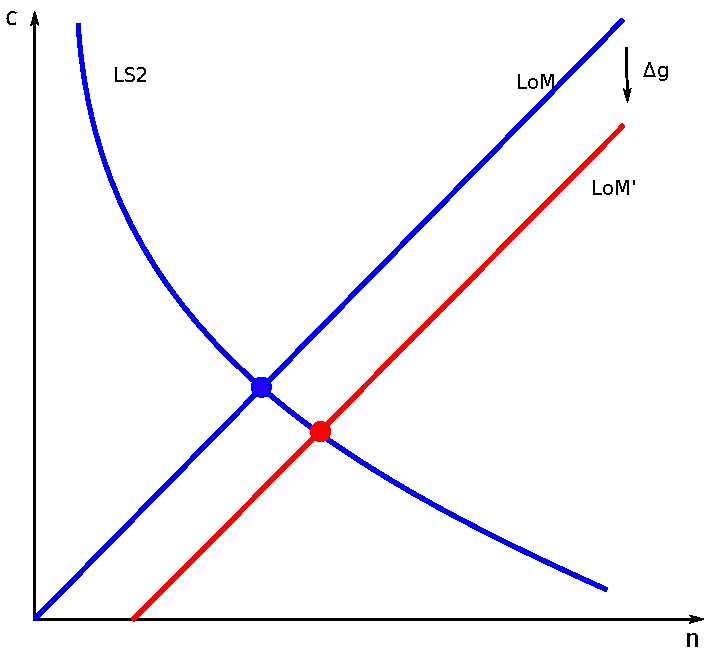
\includegraphics[scale=0.6]{lec1_fig0}
        \par\end{centering}
        \caption{Permanent increase in government purchases.}
        \end{figure}
        
        \end{frame}
        %
        \begin{frame}{Multiplier - long run}
        \begin{itemize}
        \item Note 
        \[
        \frac{dy}{dg}=F\left(\eta,1\right)\frac{\partial n\left(g\right)}{\partial g}
        \]
        \item Key: response of labor supply to $g$.
        \item To get $\partial n\left(g\right)/\partial g$ define 
        \[
        H\left(n,g\right)\equiv\phi\left(n,F_{2}\left(\eta,1\right)\right)-\left(F\left(\eta,1\right)-\eta\delta\right)n+g
        \]
        and apply Implicit Function Theorem to obtain 
        \[
        \frac{\partial n\left(g\right)}{\partial g}=\frac{1}{\left(F\left(\eta,1\right)-\eta\delta\right)-\phi_{1}\left(n,F_{2}\left(\eta,1\right)\right)}
        \]
        with $\phi_{1}\left(n,F_{2}\left(\eta,1\right)\right)=\frac{v''\left(n\right)}{u''\left(c\right)F_{2}\left(\eta,1\right)}$
        \end{itemize}
        \end{frame}
        %
        \begin{frame}{Multiplier - long run}
        \begin{itemize}
        \item We can rewrite the multiplier (verify!) as
        \[
        \frac{dy}{dg}=\frac{1}{1-\frac{i}{y}+\frac{c}{y}\frac{1}{\varphi\theta}},
        \]
        which depends on observable ratios (investment-to-output and consumption-to-output)
        and the utility function evaluated at the steady state, $\varphi\equiv\frac{v'\left(n\right)}{v''\left(n\right)n},\,\theta\equiv-\frac{u''\left(c\right)c}{u'\left(c\right)}$.
        \item It is
        \begin{itemize}
        \item Increasing in $\varphi$;
        \item Increasing in $\theta$;
        \item Increasing in $i/y$;
        \item Decreasing in $c/y$.
        \end{itemize}
        \end{itemize}
        \end{frame}
        %
        \begin{frame}{Multiplier - long run}
        
        \[
        \frac{dy}{dg}=\frac{1}{1-\frac{i}{y}+\frac{c}{y}\frac{1}{\varphi\theta}},
        \]
        
        \begin{itemize}
        \item Some remarks:
        \begin{itemize}
        \item It \alg{CAN} exceed 1.
        \item It \alr{equals 0} when labor supply is fixed.
        \item It \alr{cannot exceed 1} if investment is zero (for example economy with
        fixed exogenous capital or no capital).
        \item It is big when a large increase in labor supply requires a small decrease
        in consumption.
        \end{itemize}
        \item Remember: it was financed by lump sum taxes.
        \end{itemize}
        \end{frame}
        %
        \begin{frame}{Phase diagrams}
        \begin{itemize}
        \item To visualize the effects of government purchases we can use phase diagrams. 
        \item They are also useful to show short-run effects of government purchases
        (esp. in continuous time).
        \item To plot them: 
        \begin{itemize}
        \item Try to eliminate all static variables (in this model you can pick
        $n_{t}$)
        \item Think of conditions ensuring that variables do not change over time
        in terms of other variables and parameters (i.e., find conditions for
        $c_{t}=c_{t+1}$ and $k_{t}=k_{t+1}$). 
        \item Represent these conditions graphically.
        \item Think of dynamics of the system for points $\left(c,k\right)$ where
        these conditions are not satisfied.
        \item Locate the saddle path.
        \end{itemize}
        \end{itemize}
        \end{frame}
        %
        \begin{frame}[plain]
        
        \begin{figure}
        \begin{centering}
        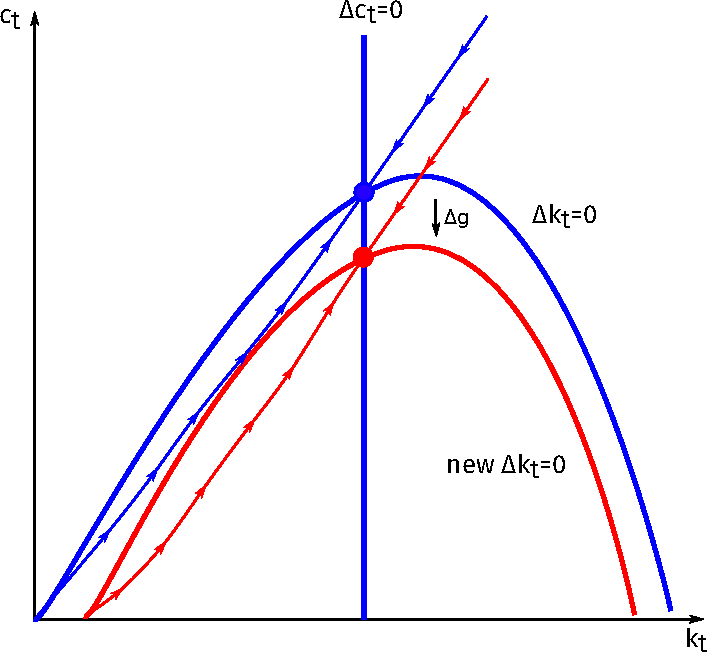
\includegraphics[scale=0.6]{lec1_fig2}
        \par\end{centering}
        \caption{Phase diagram: permanent increase in government purchases by $\Delta g$
        in an economy with fixed labor supply.}
        \end{figure}
        
        \end{frame}
        %
        \begin{frame}[plain]{}
        
        \begin{figure}
        \begin{centering}
        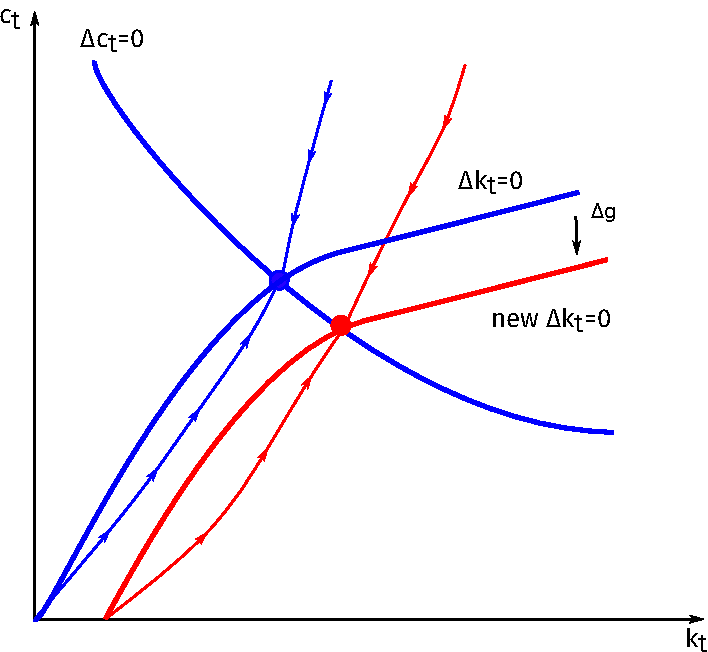
\includegraphics[scale=0.6]{lec1_fig3}
        \par\end{centering}
        \caption{Phase diagram: permanent increase in government purchases by $\Delta g$
        in an economy with flexible labor supply.}
        \end{figure}
        \end{frame}
        %
        \begin{frame}{Exercises}
        
        \begin{enumerate}
        \item Suppose $u\left(c\right)=\frac{c^{1-\theta}-1}{1-\theta}$,
        $v\left(n\right)=\frac{n^{1+\frac{1}{\varphi}}}{1+\frac{1}{\varphi}}$,
        $i/y=0.2$ and $c/y=0.6$. What is the size of the multiplier if $\theta=1$
        (log-utility) and $\varphi\in\left\{ 0,0.5,1,2,\infty\right\} $?
        \item Suppose that we have $u\left(c,n\right)=\gamma\log c+\left(1-\gamma\right)\log\left(1-n\right)$.
        Rederive the formula for the long run multiplier. 
        \item Is the adjustment to the new steady state instantaneous
        or not? What happens on impact?
        \end{enumerate}
        \end{frame}
        %
        \begin{frame}{Multiplier - long run}
        \begin{itemize}
        \item Let's analyze an economy with fixed labor supply. 
        \item In the steady state
        \begin{align}
        1 & =\beta\left[1-\delta+F_{1}\left(k,1\right)\right]\tag{EE}\label{EE-1-2}\\
        c & =F\left(k,1\right)-\delta k-\al{g}\tag{LoM}\label{LoM-1-2}
        \end{align}
        \item Notice $g$ does not enter (EE). It does not affect incentives to
        save. Investment is not affected. 
        \item $k$ remains the same and because it is the only factor of production
        in this economy output does not change. We have \alr{$dc=-dg$}.
        \item \alr{Government purchases crowd out private consumption one to one.}
        \item Remember that lump-sum tax $T$ has to be raised to finance $g$.
        It reduces HH's wealth. 
        \end{itemize}
        \end{frame}
        %
        \begin{frame}{Transition}
        \begin{itemize}
        \item We will study transition to the new steady state using phase diagrams.
        \item In discrete time it is a bit awkward, but we still can get some insight.
        \item Here we analyze unexpected permanent shocks.
        \item To proceed 
        \begin{itemize}
        \item Locate the new saddle path.
        \item Plot arrows representing trajectories.
        \item Make sure the economy jumps to the new saddle path on impact.
        \item Very important: identify variables that \alr{CANNOT} jump (almost
        always capital).
        \item After the shock the economy follows the new saddle path to the new
        steady state.
        \end{itemize}
        \end{itemize}
        
        \end{frame}
        %
        \begin{frame}{Transition}
        
        \begin{figure}
        \begin{centering}
        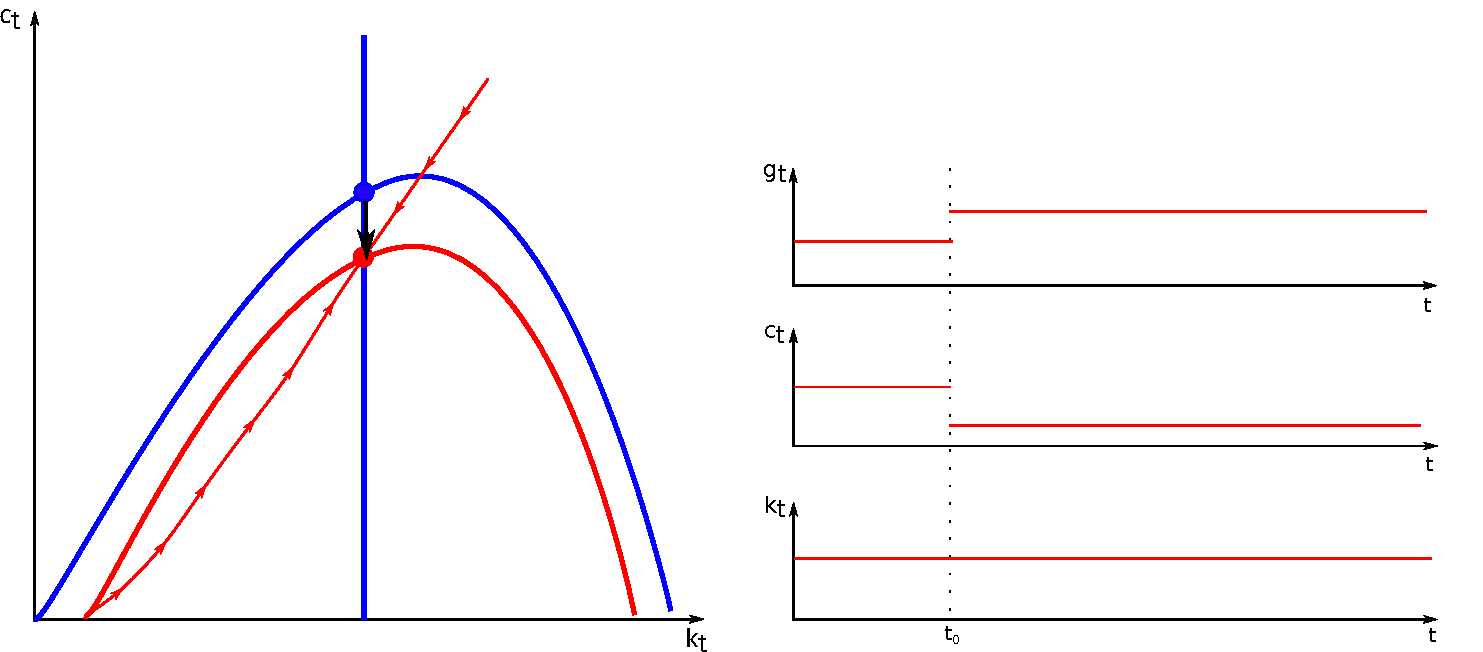
\includegraphics[scale=0.6]{lec1_fig2_transition}
        \par\end{centering}
        \caption{Phase diagram: permanent increase in government purchases by $\Delta g$
        in an economy with fixed labor supply: transition}
        \end{figure}
        
        \end{frame}
        %
        \begin{frame}{Transition}
        
        \begin{figure}
        \begin{centering}
        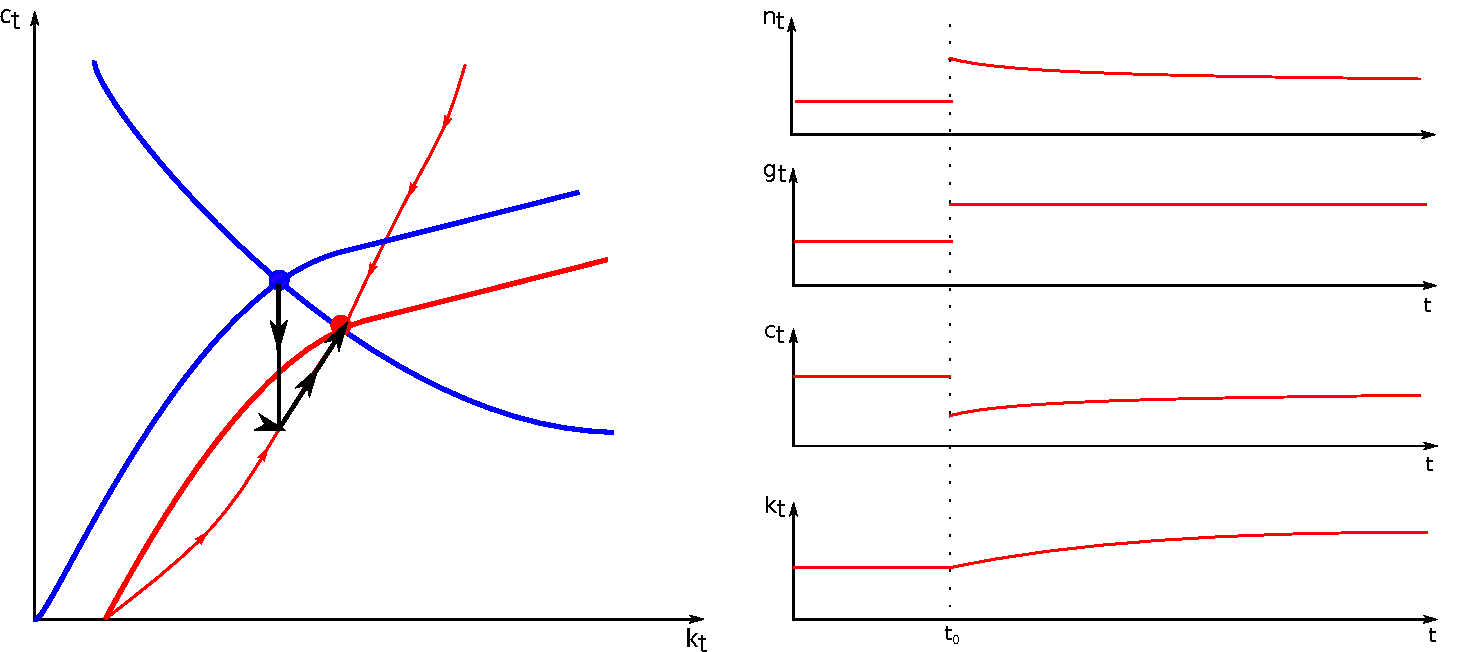
\includegraphics[scale=0.6]{lec1_fig3_transition}
        \par\end{centering}
        \caption{Phase diagram: permanent increase in government purchases by $\Delta g$
        in an economy with flexible labor supply: transition}
        \end{figure}
        
        \end{frame}
        %
        
        \section*{Government purchases multiplier: short run}
        \begin{frame}{Multiplier - short run}
        
        \begin{itemize}
        \item More interesting exercise: temporary increase in $g$. For simplicity
        we start in the steady state with $g_{t}=g$ and consider an unexpected
        increase in $g_{0}$ that lasts for some periods.
        \item Think of a war or a stimulus package based on government purchases.
        \item Main result: \alr{difficult to generate $dy_{0}/dg_{0}>1$} in a baseline
        NGM. Why?
        \item After discussing theoretical results we will look at empirical findings.
        \end{itemize}
        \end{frame}
        %
        \begin{frame}{Multiplier - short run}
        
        \begin{itemize}
        \item What happens after $g_{0}$ goes up? 
        \begin{itemize}
        \item $k_{0}$ is fixed.
        \item $y_{0}$ can grow only if $n_{0}$ increases.
        \end{itemize}
        \item (LS) implies that 
        \[
        v'\left(n_{0}\right)=u'\left(c_{0}\right)F_{2}\left(k_{0},n_{0}\right)\tag{LS}
        \]
        so given our assumptions $n_{0}$ can increase \alr{only} if $c_{0}$
        does not increase. 
        \end{itemize}
        \end{frame}
        %
        \begin{frame}{Multiplier - short run}
        \begin{itemize}
        \item $c_{0}$ has to fall (or at least not increase). When is it possible?
        Recall (EE)
        \[
        \frac{u'\left(c_{0}\right)}{u'\left(c_{1}\right)}=\beta\left[1-\delta+F_{1}\left(k_{1},n_{1}\right)\right]
        \]
        \item We need $u'\left(c_{0}\right)/u'\left(c_{1}\right)>1$. Intuitively,
        the economy has to return to the steady state eventually (formally:
        TVC). This can happen only if 
        \[
        \beta\left[1-\delta+F_{1}\left(k_{1},n_{1}\right)\right]>1
        \]
        so the interest rate $r_{1}\coloneqq F_{1}\left(k_{1},n_{1}\right)-\delta$
        has to be higher than in the steady state.
        \item Remember: behavior of consumption determined by the real interest rate. 
        \end{itemize}
        \end{frame}
        %
        \begin{frame}{Multiplier - short run}
        \begin{itemize}
        \item This is possible if $k_{1}/n_{1}<k/n$. So, unless $n_{1}>n$, $k_{1}<k_{0}$.
        \item This requires fall in investment.
        \item To have $dy_{0}/dg_{0}>1$ we need more persistent shocks and high
        $\varphi$. Recall when permanent increase in $g$ does not crowd
        out consumption.
        \end{itemize}
        \end{frame}
        %
        \begin{frame}{Multiplier - short run}
        \begin{itemize}
        \item In a standard NGM it is hard to get multipliers exceeding 1.
        \item With standard calibration $dy_{0}/dg_{0}$ is rather low. 
        \item Suppose
        $$u\left(c\right)=\log c, \quad v\left(n\right)=\kappa\frac{n^{1+\frac{1}{\varphi}}}{1+\frac{1}{\varphi}}$$
        and parameter values be 
        \begin{table}
        \centering{}%
        \begin{tabular}{|c|c|c|c|}
        \hline 
        $\delta$ & $\beta$ & $\alpha$ & $\frac{g}{y}$\tabularnewline
        \hline 
        \hline 
        0.02 & 0.99 & 1/3 & 0.2\tabularnewline
        \hline 
        \end{tabular}
        \end{table}
         and $n=1$ in the steady state.
        \end{itemize}
        \end{frame}
        %
        \begin{frame}[plain]{}
        
        \begin{figure}
        \begin{centering}
            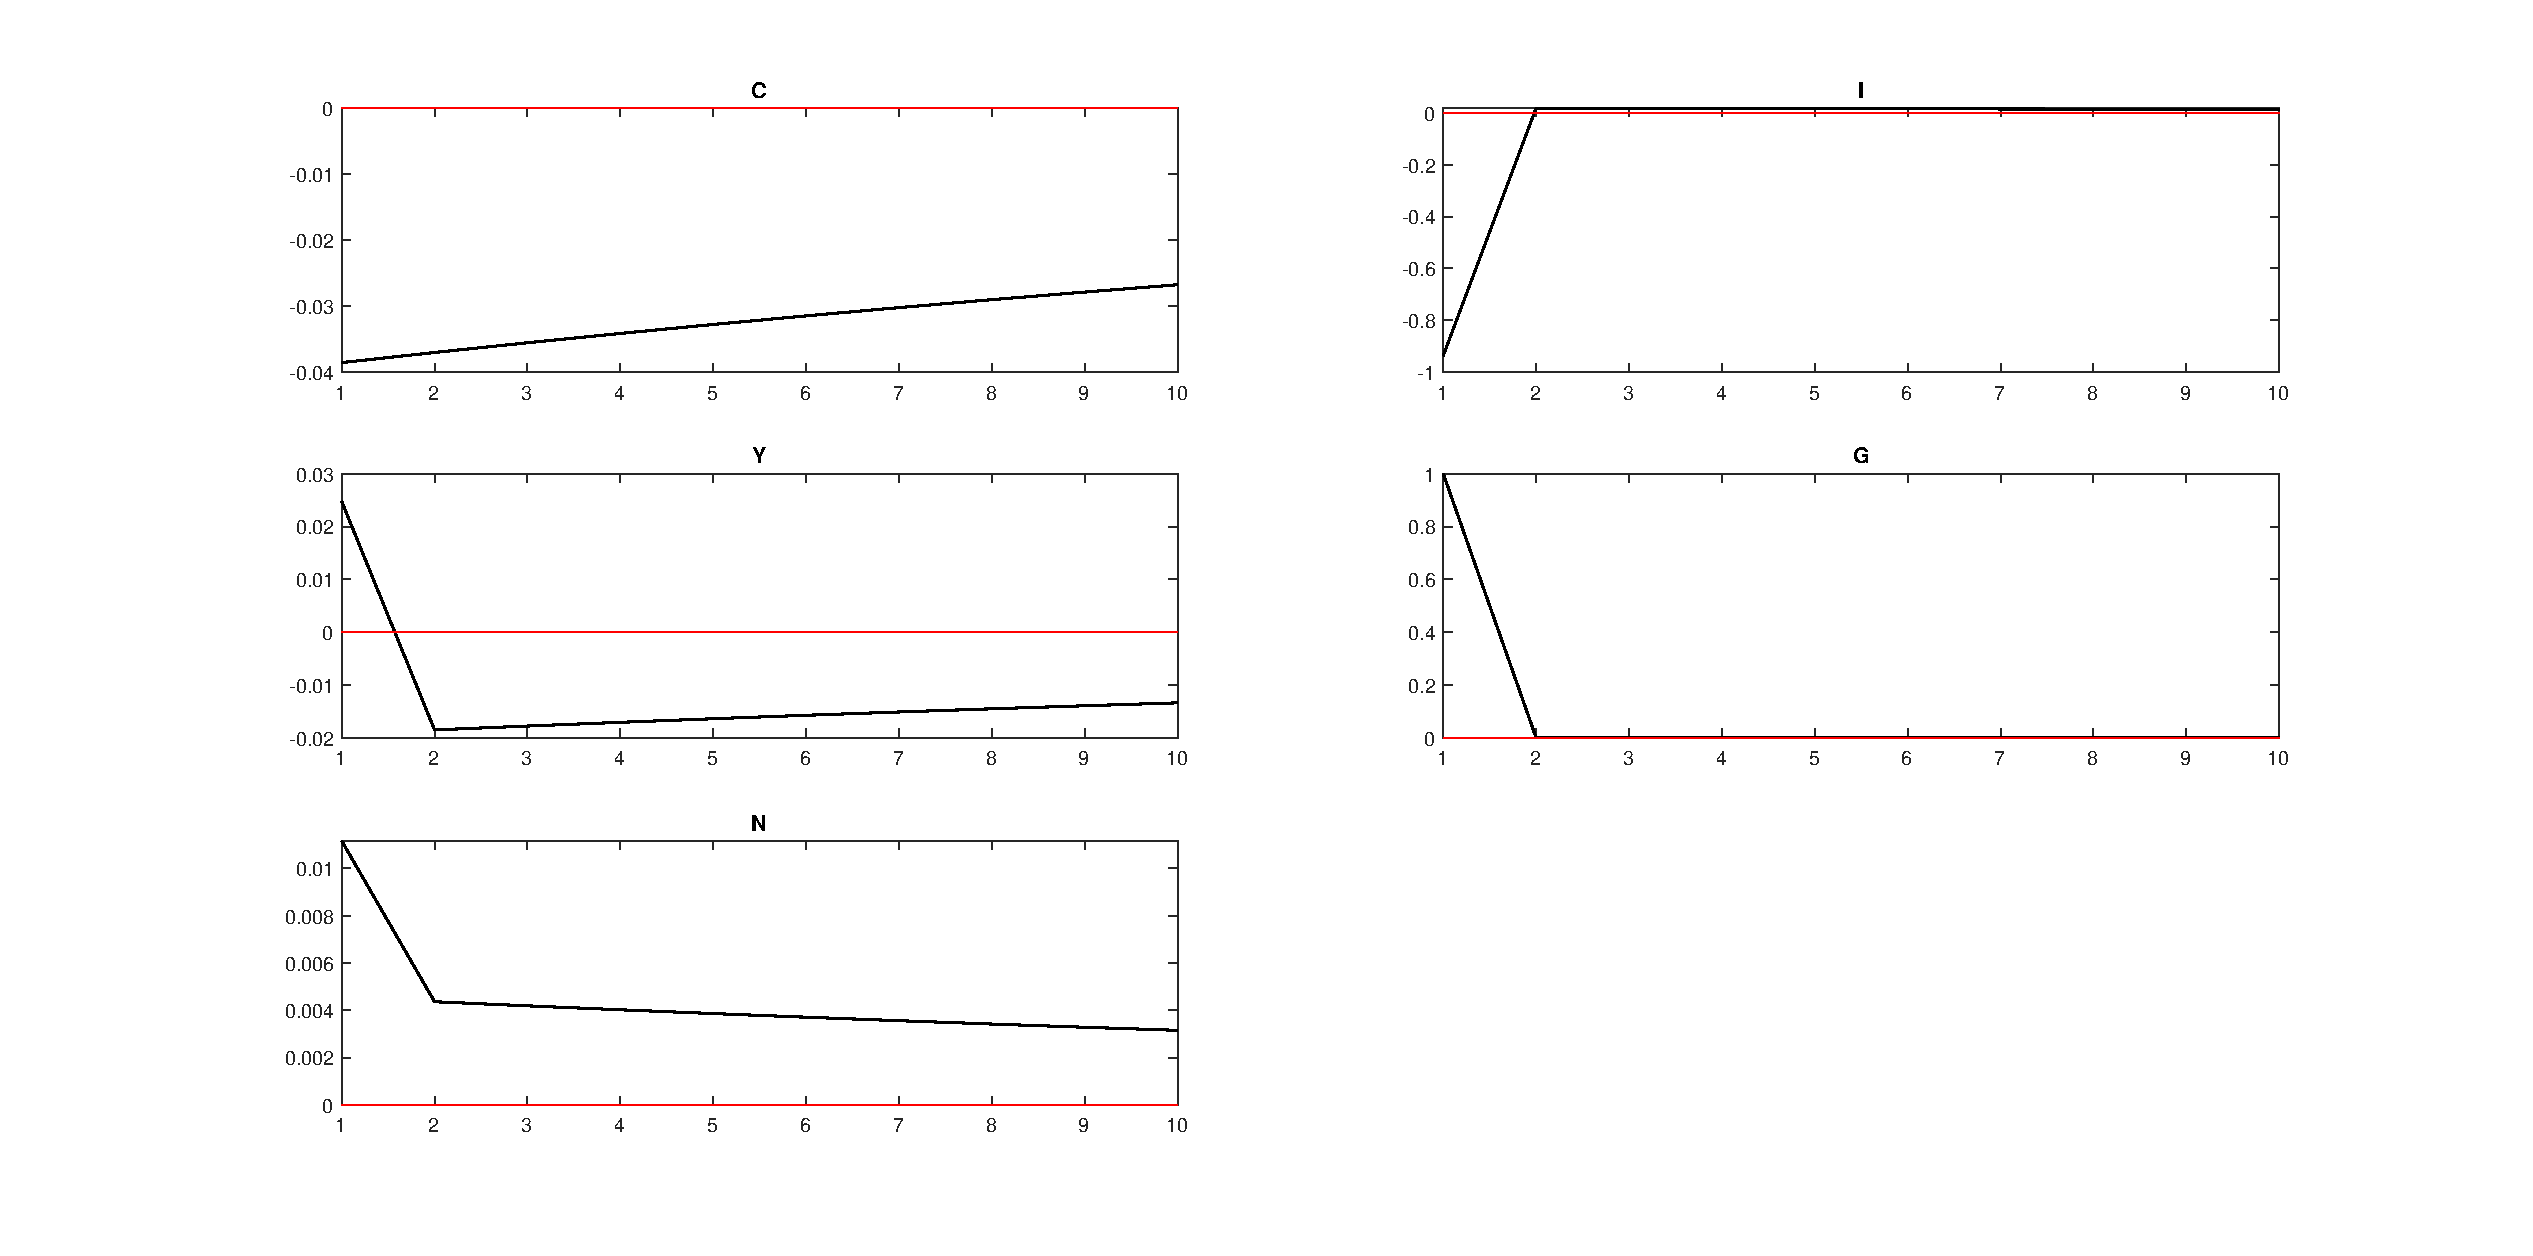
\includegraphics[scale=0.38]{multiplier1.eps}
        \par\end{centering}
        \caption{Dynamics after an unexpected increase in $g$: $\varphi=1$}
        \end{figure}
        
        \end{frame}
        %
        \begin{frame}[plain]{}
        
        \begin{figure}
        \begin{centering}
            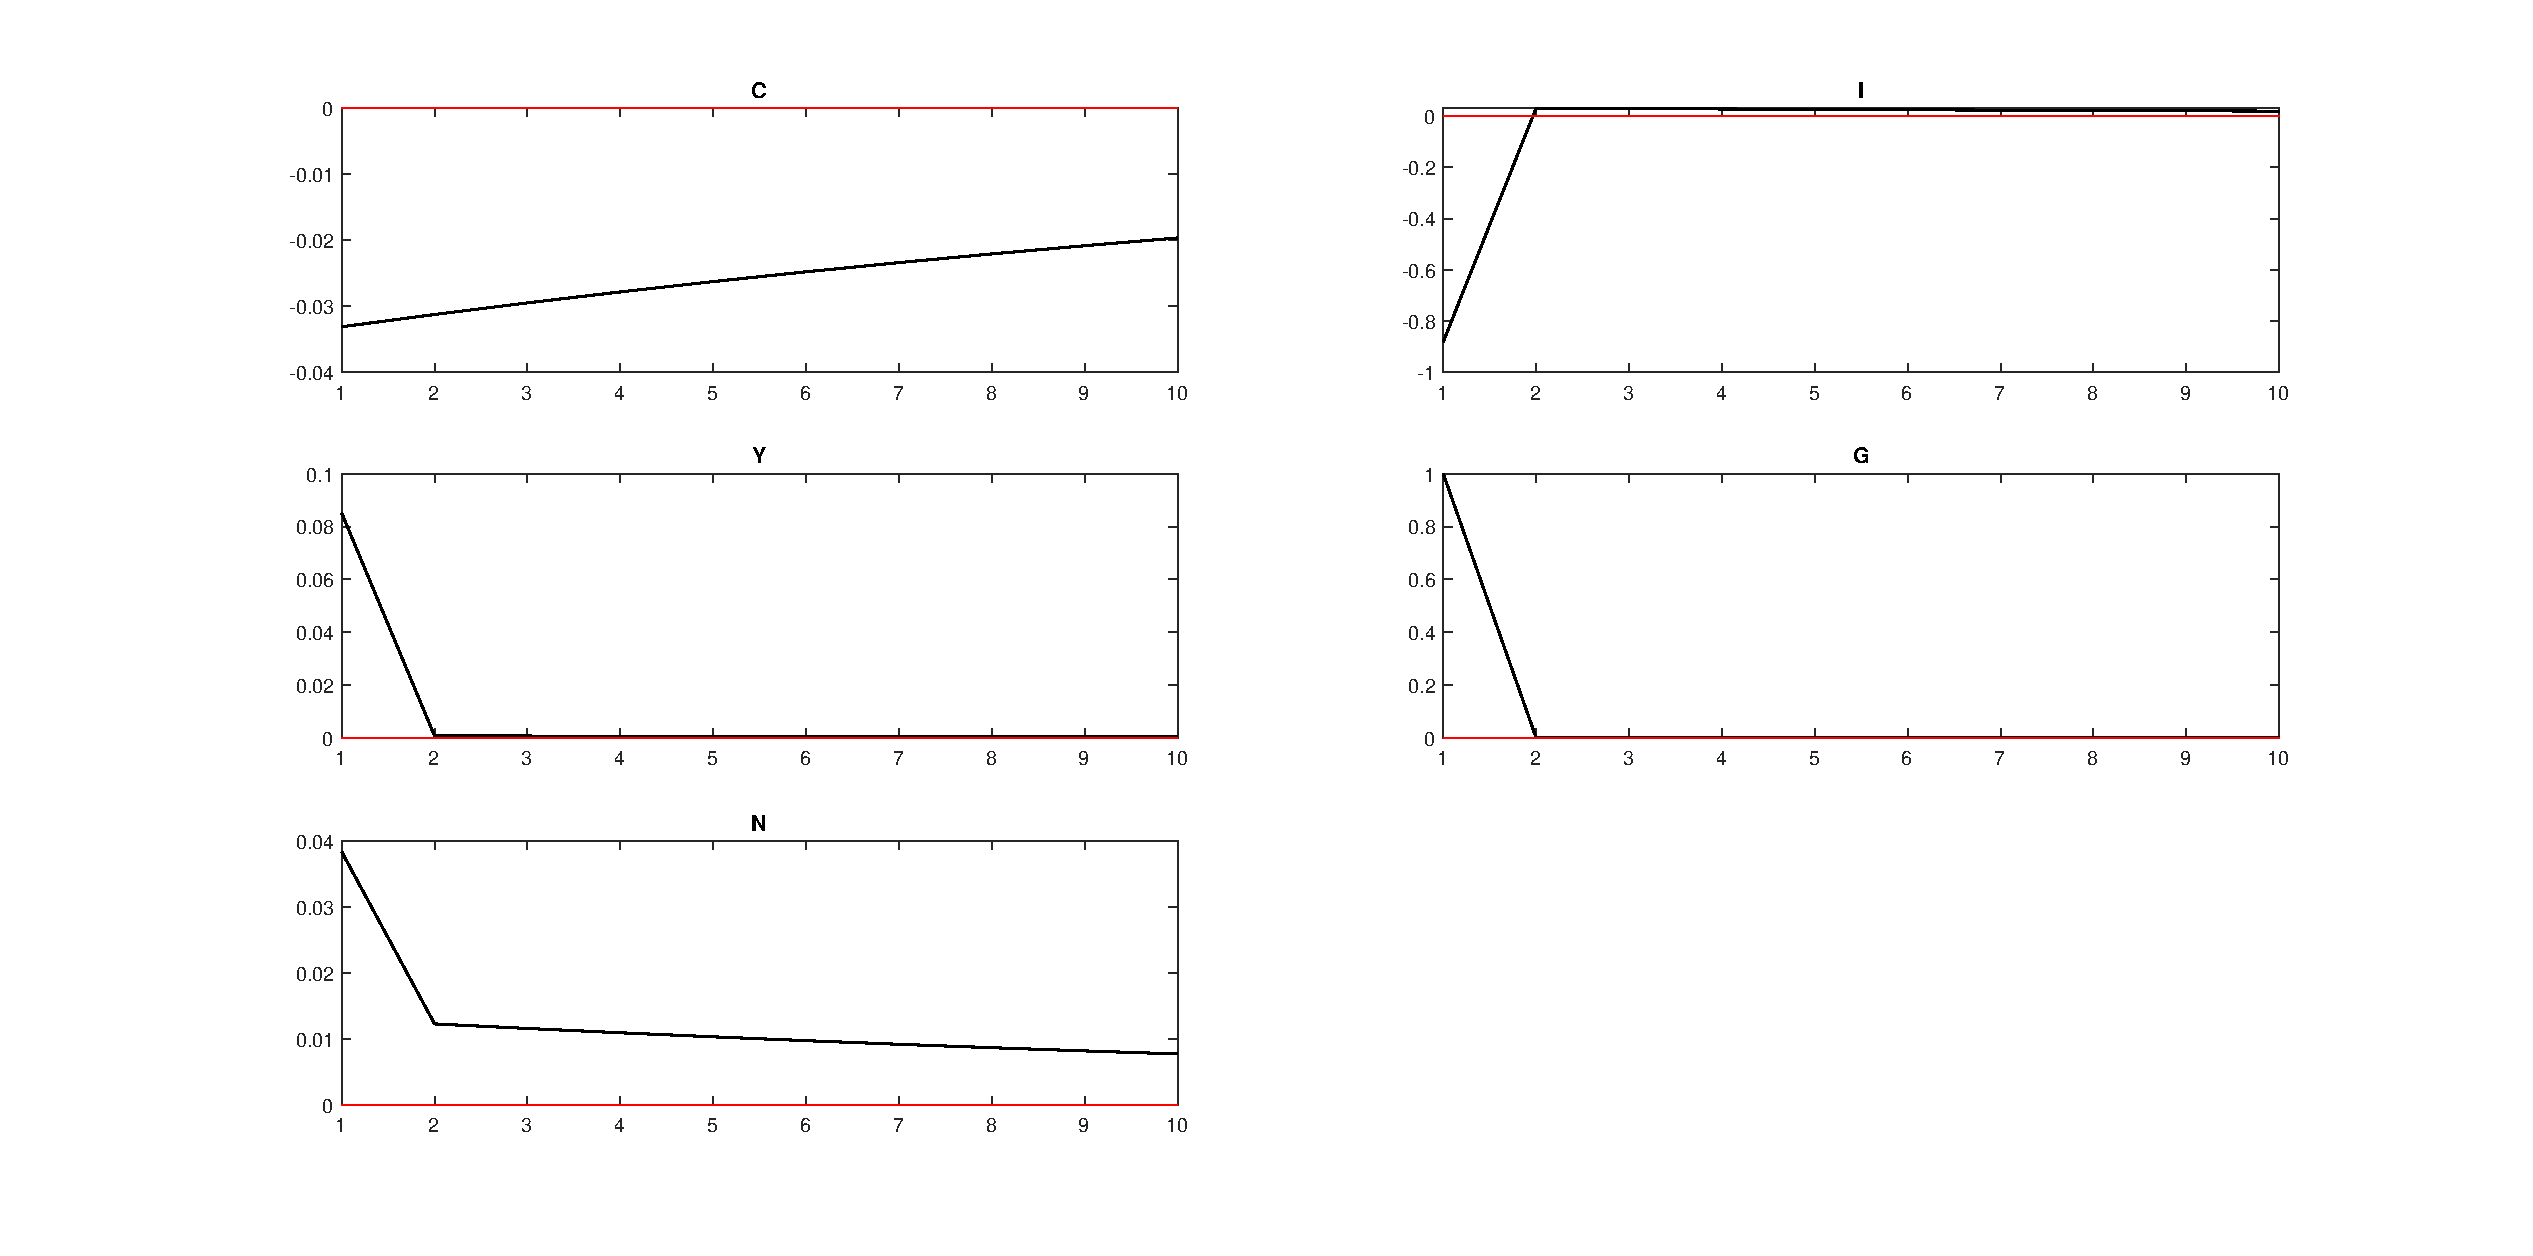
\includegraphics[scale=0.38]{multiplier2_highfrisch.eps}        \par\end{centering}
        \caption{Dynamics after an unexpected increase in $g$: $\varphi=\infty$}
        \end{figure}
        
        \end{frame}
        %
        \begin{frame}[plain]{}
        
        \begin{figure}
        \begin{centering}
            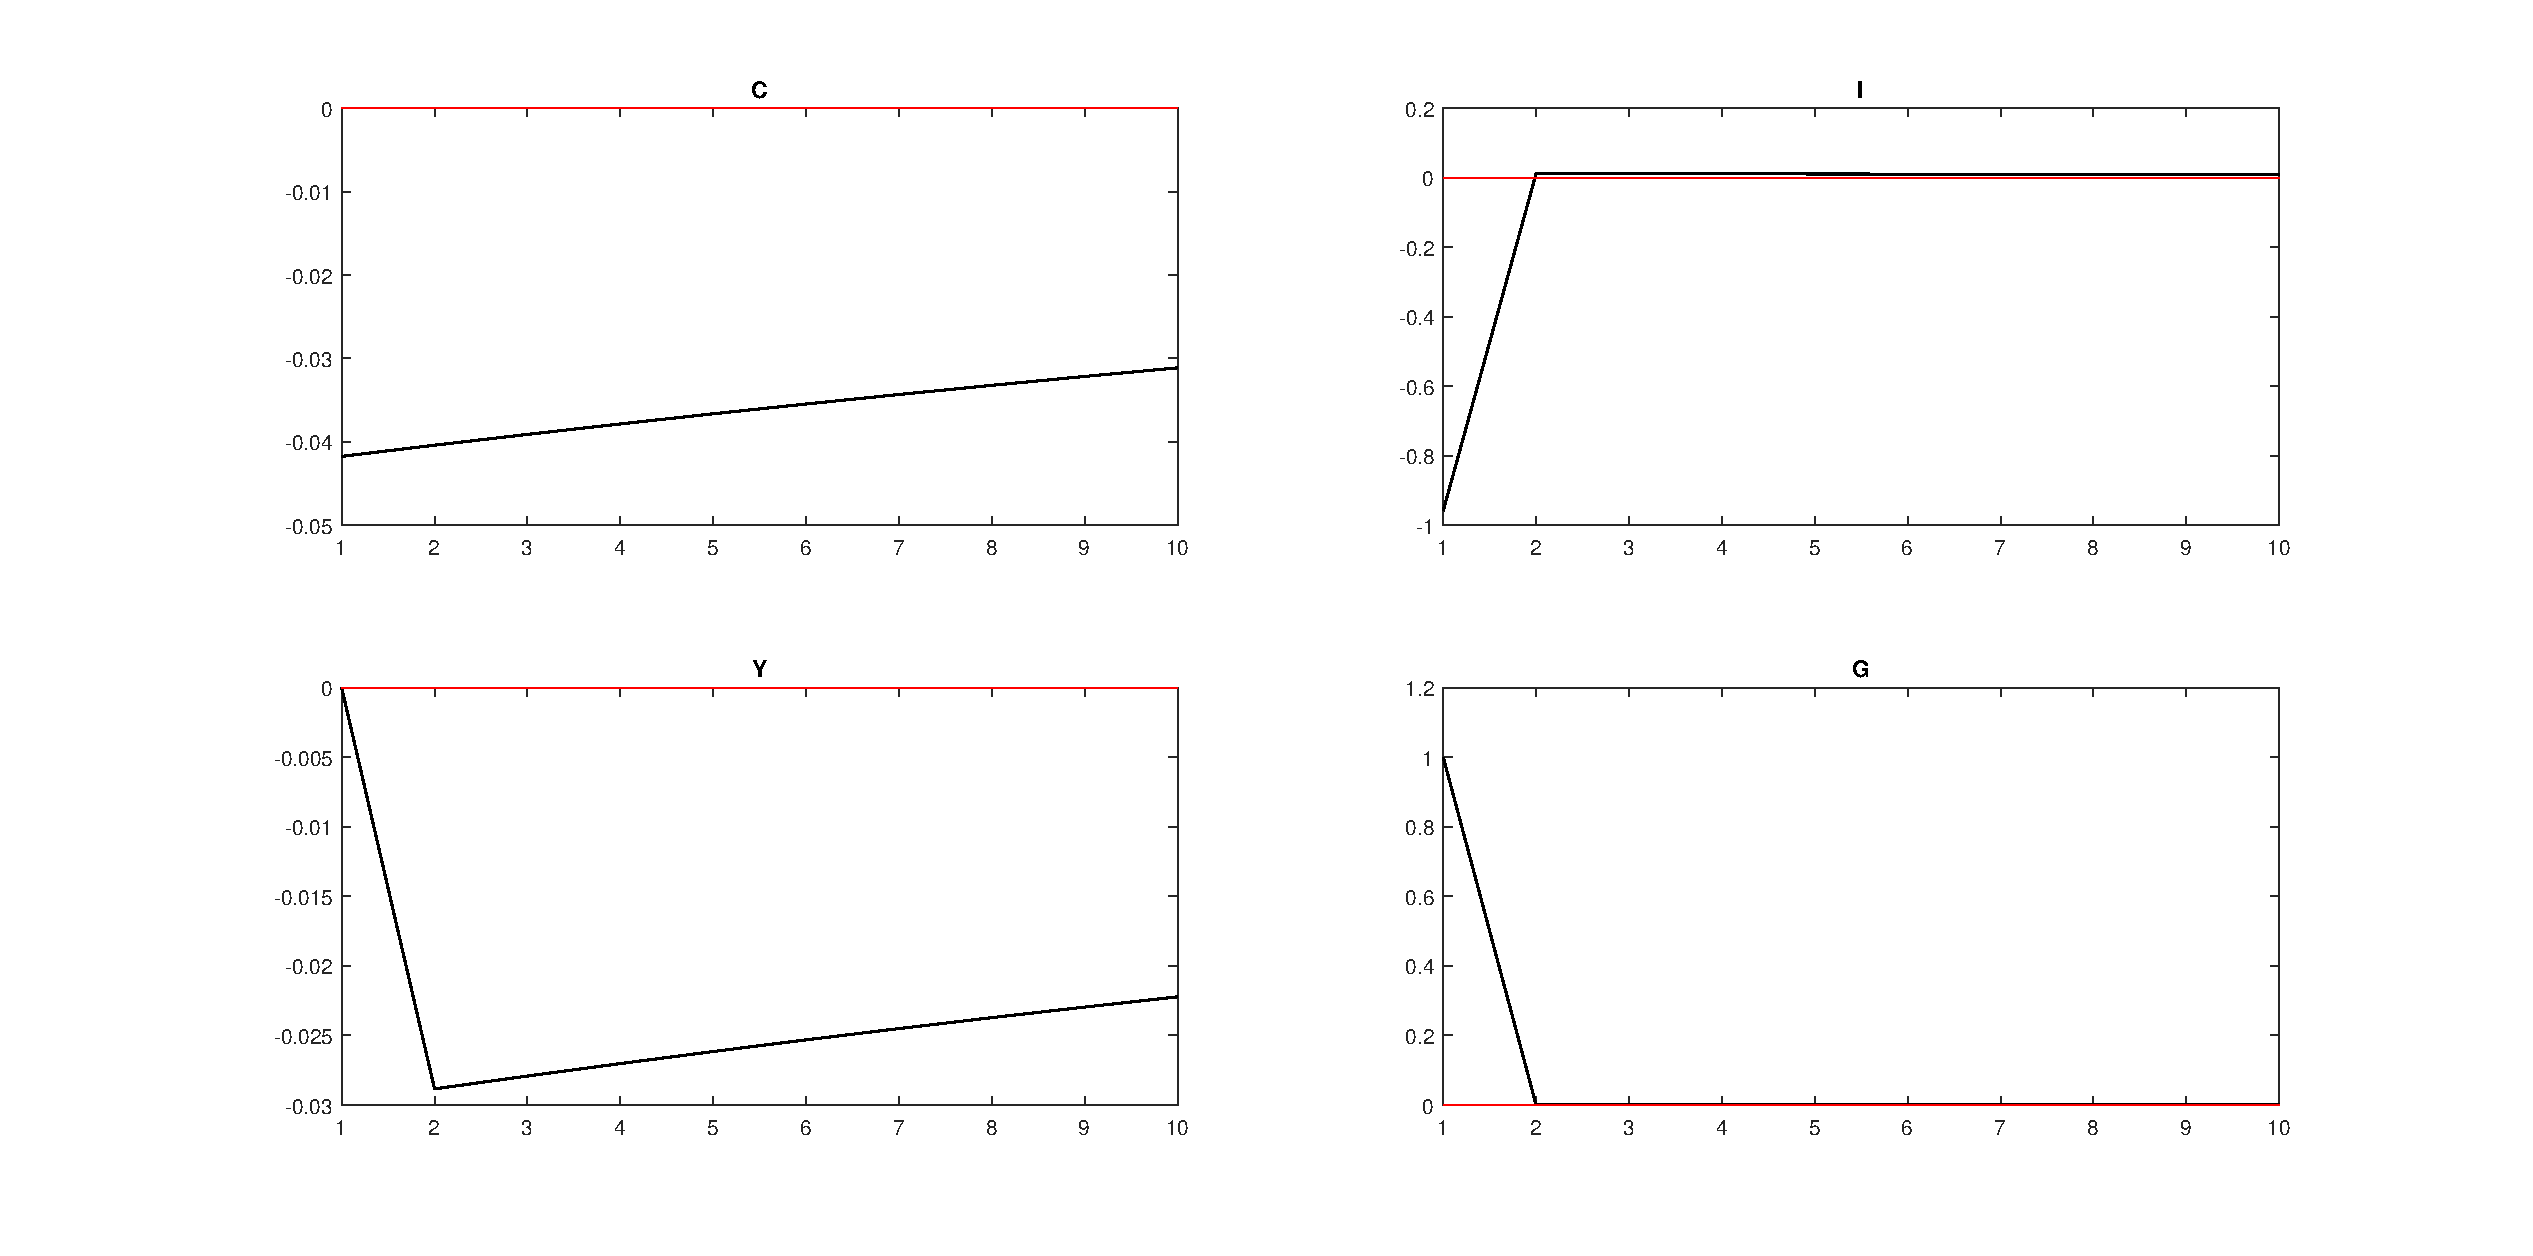
\includegraphics[scale=0.38]{multiplier2_lowfrisch.eps}               \par\end{centering}
        \caption{Dynamics after an unexpected increase in $g$: $\varphi=0$}
        \end{figure}
        
        \end{frame}
        %
        \begin{frame}[plain]{}
        
        \begin{figure}
        \begin{centering}
            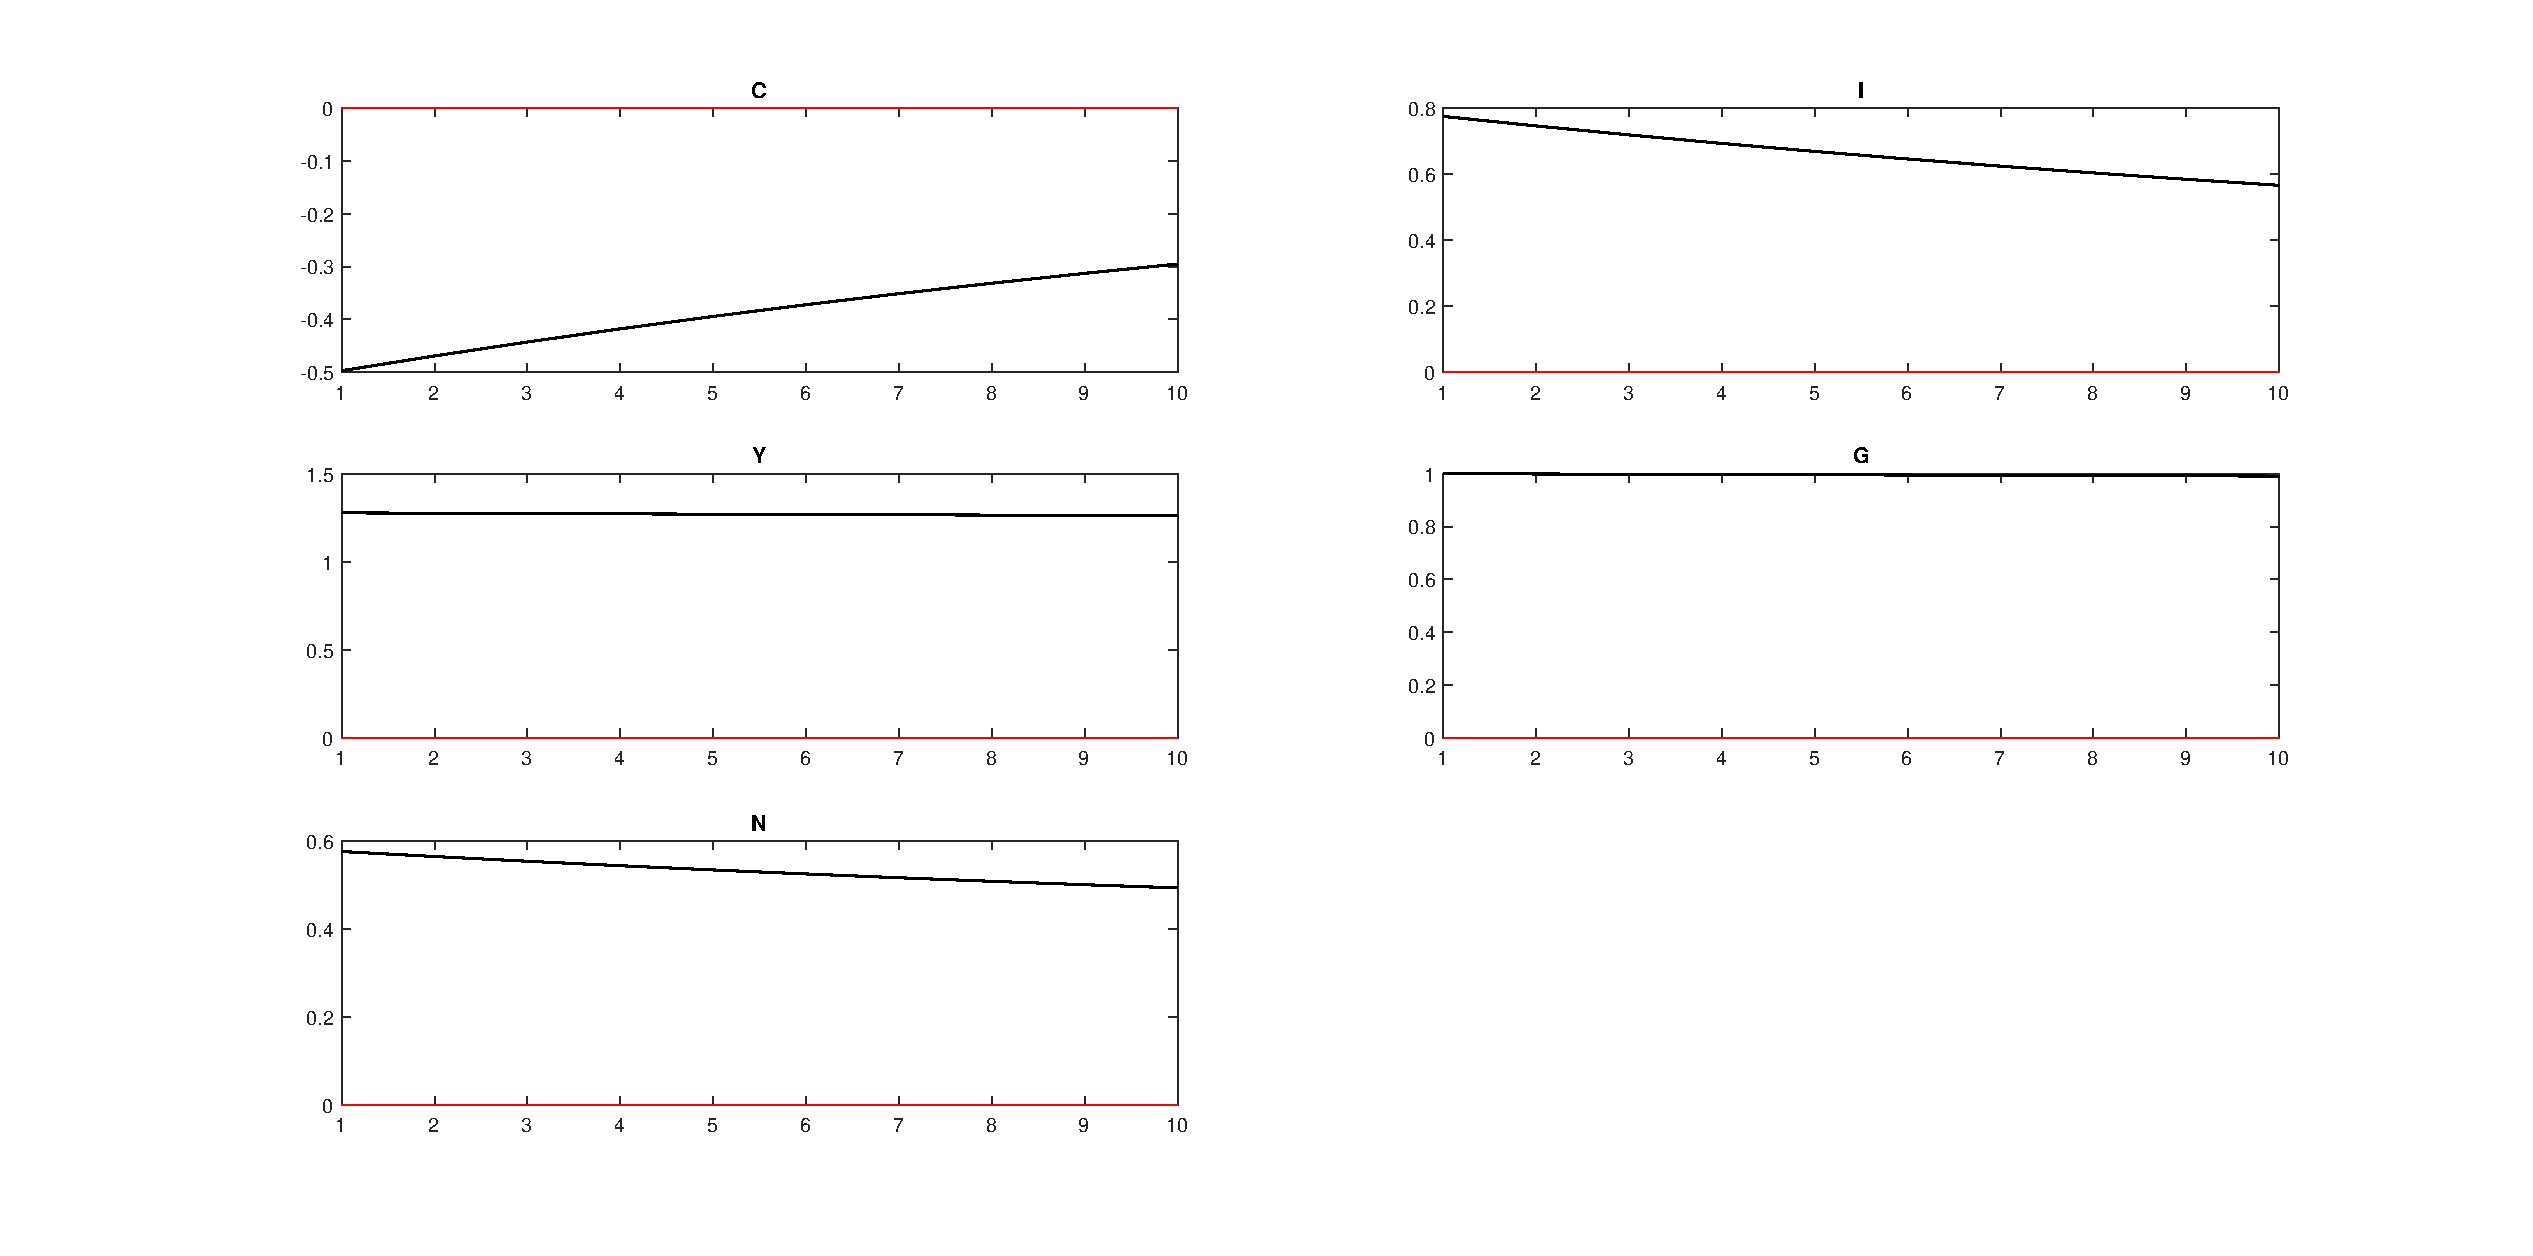
\includegraphics[scale=0.38]{multiplier_persistenthighfrisch.eps}       
            \par\end{centering}
        \caption{Dynamics after an unexpected increase in $g$: $\varphi=\infty$ and
        very persistent increase in $g$ (almost permanent)}
        \end{figure}
        
        \end{frame}
        %

     

\end{document}